% !TEX root = Sotsuron_main_v3.tex
%%Chap3
テキストを集合の要素とした類似検索にはEfstathiadesらが扱ったSTPSJoin問題\cite{efstathiades}がある.STPSJoin問題は静的なテキスト集合から類似するユーザペアの集合を検索するJoin問題である.一方でCTS問題は動的なテキスト集合を扱い,クエリとなるユーザと類似度が閾値以上であるユーザを検索する点が異なる.また,STPSJoin問題の類似度は相手のユーザが持つテキストの中に類似するテキストが一つでもあるテキストの数の割合である.一方でCTS問題の類似度は類似するテキストのペア同士で辺を結ぶことで構築される二部グラフの極大マッチングのサイズである.このように類似度の求め方も異なる.
本章では,久保らが提案したCTS問題に対する類似検索アルゴリズムである遅延評価法を説明する.遅延評価法の疑似コードをAlgorithm \ref{alg:statedelay}に示す.この遅延評価法はマッチング判定を行う際,ユーザ間類似度を正確に求めるのではなく,ユーザ間類似度が$\epsilon_u$を越えるかのみを調べることによってマッチング判定回数の削減を行い,高速化を狙ったアルゴリズムである.
遅延評価法では以下のようにクエリユーザ$V$のスライディングウィンドウ$V_{T}$内のそれぞれのテキストを以下の3つの集合に分類する.
\begin{itemize}
  \item $V_{M}$ マッチングすることが確定したテキスト集合
  \item $V_{NM}$ マッチングしないことが確定したテキスト集合
  \item $V_{UM}$ マッチングするか未定なテキスト集合
\end{itemize}
さらに,ユーザごとにスライディングウィンドウ$U_{T}$内のそれぞれのテキストを以下の2つの集合に分類する.
\begin{itemize}
  \item $U_{M}$ マッチングすることが確定したテキスト集合
  \item $U_{UM}$ マッチングするか未定なテキスト集合
\end{itemize}

%そのために,以下の二つを行う.
以上の定義より$|V_M|=|U_M|$が成り立つ.
\begin{itemize}
    \item 「マッチングすることが確定した」とはただ1つのテキストとペアになっている状態を指す.
    \item 「マッチングしないことが確定した」とはペアになるための条件を満たすテキストが1つも存在しない状態を指す.つまりマッチングペアの対象のすべてのテキストとのJaccard類似度は計算済みである.
    \item 「マッチングするか未定」とはマッチングペアの対象のすべてのテキストとのJaccard類似度の算出が済んでいない状態であり,マッチングする可能性が残っているテキストという意味である.
\end{itemize}

この遅延評価法は,
\begin{itemize}
    \item 類似となる条件 $|V_M|\geq\epsilon_u$
    \item 非類似となる条件 $|V_{NM}|>W-\epsilon_u$
\end{itemize}
のどちらかの条件を満たすまでマッチング判定をすることによって必要以上のマッチング判定処理を省き,ユーザ間類似度が閾値$\epsilon_u$以上になるユーザを効率よく見つけ出すことを狙っている.
遅延評価法の処理の流れを図\ref{fig:lazy}に示す.
$V$,$U$のスライディングウィンドウに入ってくるテキストを$\mbox{IN}_V$,$\mbox{IN}_U$,スライディングウィンドウから離脱するテキストを$\mbox{OUT}_V$,$\mbox{OUT}_U$とする.
\begin{figure}[htb]
    \centering
    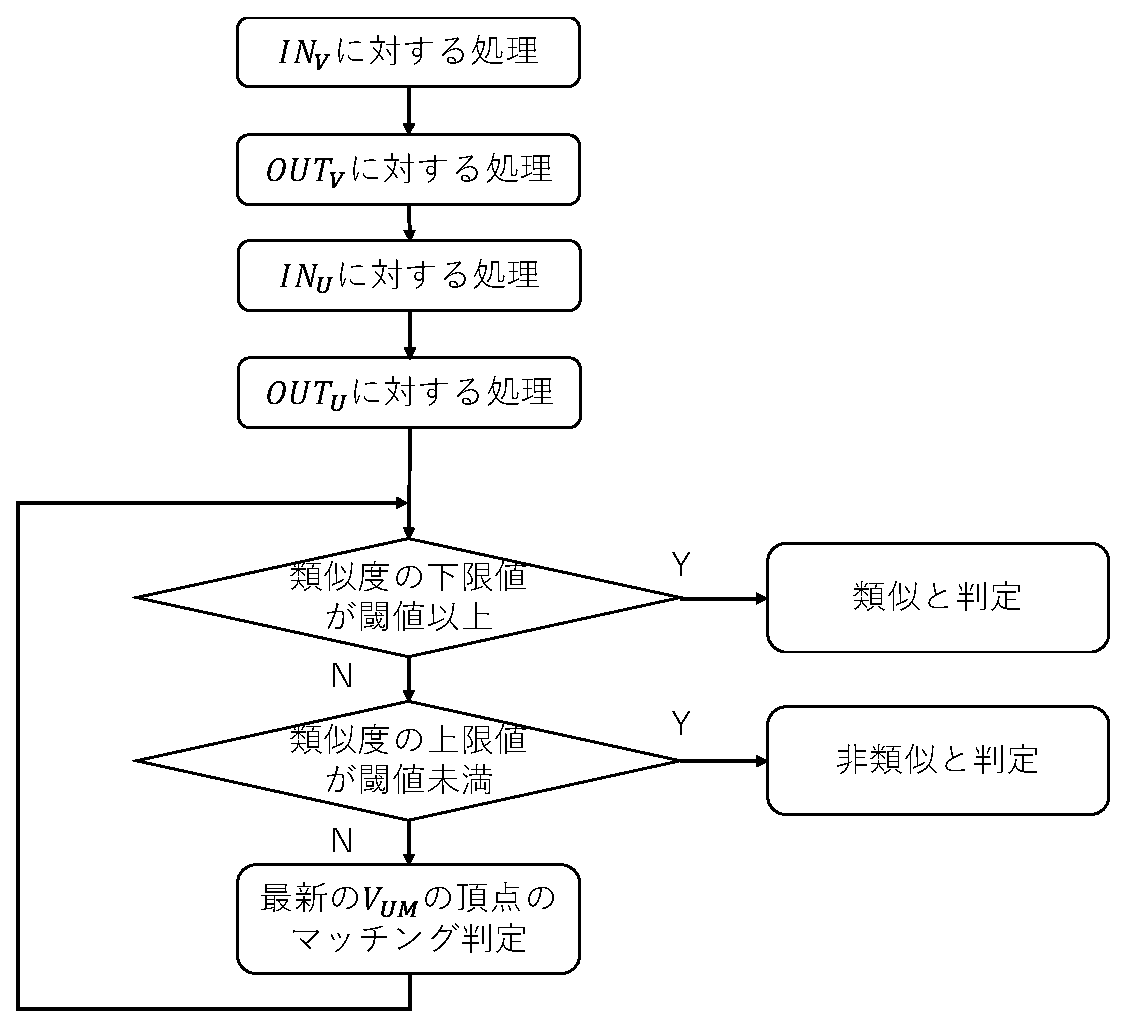
\includegraphics[width=8.7cm]{img/delay.eps}
    \caption{遅延評価法の処理の流れ}
    \label{fig:lazy}
\end{figure}

\section{\texorpdfstring{$\mbox{IN}_{V}$} に対する処理}
クエリ$V$のテキストストリームに新しいテキスト$\mbox{IN}_V$が到着し,$\mbox{IN}_V \in V_{UM}$とする.

\section{\texorpdfstring{$\mbox{OUT}_V$} に対する処理}
最も古いテキスト$\mbox{OUT}_V$を$V_M$,$V_{NM}$,$V_{UM}$の所属している集合から除外する.特に$\mbox{OUT}_V \in V_{M}$であった時は,$\mbox{OUT}_V$のマッチング相手であったユーザ$U$のテキスト$O_U$はマッチング相手がいなくなることから$O_U$を$U_{M}$から除外する.さらに,$O_U$は$V_{NM}$のテキストとマッチングする可能性があるため,$O_U$と$V_{NM}$のテキストとのマッチング判定を行う.
\begin{itemize}
    \item $V_{NM}$内のテキスト$O_V$とマッチングした場合 : $O_V \in V_{M},O_U \in U_{M}$
    \item マッチングしなかった場合 : $O_U \in U_{UM}$
\end{itemize}
とする.

\section{\texorpdfstring{$\mbox{IN}_U$} に対する処理}
ユーザ$U$のテキストストリームに新しいテキスト$\mbox{IN}_U$が到着する時,$\mbox{IN}_U$と$V_{NM}$のいずれかのテキスト同士がマッチングする可能性が発生することから,
$\mbox{IN}_U$を起点とした$V_{NM}$内の各テキストに対するマッチング判定を行う.
\begin{itemize}
    \item $V_{NM}$内のテキスト$O_V$とマッチングした場合 : $O_V \in V_{M},\mbox{IN}_U \in U_{M}$
    \item マッチングしなかった場合 : $\mbox{IN}_U \in U_{UM}$
\end{itemize}
とする.

\section{\texorpdfstring{$\mbox{OUT}_U$} に対する処理}
スライディングウィンドウ内の最も古いテキスト$\mbox{OUT}_U$を$U_M,U_{UM}$の所属している集合から除外する.特に$\mbox{OUT}_U \in U_M$であった時,$\mbox{OUT}_U$とマッチングしていたテキスト$O_V$を$O_V \in V_{UM}$とする.

\section{類似・非類似の判定処理}
ここでは各時刻Tでユーザ間類似度が$\epsilon_u$を超えるかを判定するプロセスを示している.
$V_{M}$($=U_{M}$)の大きさは常に$\mbox{sim}(V_{T},U_{T})$以下であることから,$V_{M}$の大きさがユーザ間類似度の下限値といえる.さらに$V_{NM}$に所属するテキストはマッチングすることはないため,スライディングウィンドウの大きさ$W$を用いて$W-|V_{NM}|$がユーザ間類似度の上限値となる.したがって,ユーザ間類似度を正確に求めるのではなく,類似となる条件式
\begin{equation}
\label{ruiji}
|V_{M}| \geq \epsilon_u
\end{equation}
または,非類似となる条件式
\begin{equation}
\label{hiruiji}
W - |V_{NM}| < \epsilon_u
\end{equation}
のどちらかを満たすまでマッチング判定を行えばよい.
%そこで,$|V_M| \geq \epsilon_u$,または$w-|V_{NM}| \leq \epsilon_u$のいずれかが成立するまで
そこで,式(\ref{ruiji})または式(\ref{hiruiji})のいずれかが成立するまで
%$V_{UM}$に所属するテキストを1つ取り出し,$U_{UM}$に所属するテキストとのマッチング判定を繰り返し行う.
$V_{UM}$の各テキストを起点とした$U_{UM}$内のテキストに対する以下のマッチング判定処理を繰り返し行う.

\begin{itemize}
    \item $V_{UM}$のテキスト$O_V$と$U_{UM}$のテキスト$O_U$がマッチングした場合,$O_V \in V_M,O_U \in U_M$とする.この時,$V_M$の大きさが1増加する.
    \item $V_{UM}$のテキスト$O_V$が$U_{UM}$のどのテキストともマッチングしなかった場合,$O_V \in V_{NM}$とする.このとき$V_{NM}$の大きさが1増加する.
\end{itemize}

%極大マッチングサイズの上限と下限の情報を利用して,処理の枝刈りを行い,高速化を図っている.
%データベースのテキストストリームごとに以下を設定する.



\section{マッチング判定を行うペアの順番}
\label{order_matching}
ユーザ間類似度を求める際に行うマッチング判定は,$V_{UM}$内のテキストと$U_{UM}$内のテキスト同士でマッチング判定を行うが,それぞれの集合内のどのテキストからマッチング判定を行うかは自由度が存在する.そこで遅延評価法では常に新しいテキストから優先してマッチング判定を行う.このとき,新しいテキスト同士がマッチングすることで長時間マッチングの関係が維持でき,どちらか片方のテキストがスライディングウィドウを離脱したときのマッチング判定のやり直しの回数の削減が見込める.
  %\item 古いテキストほどマッチング判定対象になりにくく,マッチング判定をされないままスライディングウィンドウを離脱するテキストが増えると考えられ,マッチング判定回数の削減が見込める.
%\end{itemize}
%ということがあげられる.

\begin{comment}
\begin{figure}[!t]
\begin{algorithm}[H]
    \caption{遅延評価法}
    \label{alg1}
    \begin{algorithmic}[1]
    \STATE $\mbox{IN}_V\in V_{UM}$とする
    \STATE $\mbox{OUT}_V$をスライディングウィンドウから離脱させる
    \IF {$\mbox{OUT}_V\in V_{M}$}
        \STATE $O_U\leftarrow Pair(\mbox{OUT}_V)$
        \FOR {$O_V\in V_{NM}$}
            \IF {($\tau(O_V,O_U)\geq \epsilon_{doc}$)}
                \STATE $O_V$と$O_U$がマッチング
                \STATE break
            \ENDIF
        \ENDFOR
    \ENDIF
    \FOR {$O_V\in V_{NM} $}
        \IF {($\tau(O_V,\mbox{IN}_U)\geq \epsilon_{doc}$)}
            \STATE $O_V$と$\mbox{IN}_U$がマッチング
            \STATE break
        \ENDIF
    \ENDFOR
    \STATE $\mbox{OUT}_U$をスライディングウィンドウから離脱させる
    \IF{$\mbox{OUT}_U\in U_{M}$}
        \STATE $Pair(\mbox{OUT}_U)\in V_{UM}$とする
    \ENDIF
    \WHILE {$|V_M| < \epsilon_u$ AND $|V_{NM}| \leq (w-\epsilon)$}
        \STATE $O_V \leftarrow V_{UM} $の一番新しいテキスト
        \FOR{$O_U \in U_{UM}$}
            \IF {($\tau(O_V,O_U)\geq \epsilon_{doc}$)}
               \STATE $O_V$と$O_U$がマッチング
            \STATE break
            \ENDIF
        \ENDFOR
        \IF{$O_V$がどの$U_{UM}$ともマッチングしない}
            \STATE $O_V\in V_{NM}$とする
        \ENDIF
    \ENDWHILE
    \IF {($|V_M|  < \epsilon_u$)}
        \STATE Not Similar
    \ENDIF
    \IF {($|V_M|  \geq \epsilon_u$)}
        \STATE Similar
    \ENDIF
\end{algorithmic}
\end{algorithm}
\end{figure}
\end{comment}



\begin{algorithm}[H]
 \caption{遅延評価法}
 \label{alg:statedelay}
 \begin{algorithmic}[1]
  \State $\mbox{IN}_V\in V_{UM}$とする
  \State $\mbox{OUT}_V$をスライディングウィンドウから離脱させる
  \If {$\mbox{OUT}_V\in V_{M}$}
    \State $O_U\leftarrow Pair(\mbox{OUT}_V)$
    \For {$O_V\in V_{NM}$}
    \If {($jac(O_V,O_U)\geq \epsilon_{doc}$)}
      \State $O_V$と$O_U$がマッチング
      \State break
    \EndIf
    \EndFor
  \EndIf
  \For {$O_V\in V_{NM} $}
  \If {($jac(O_V,\mbox{IN}_U)\geq \epsilon_{doc}$)}
  \State $O_V$と$\mbox{IN}_U$がマッチング
  \State break
  \EndIf
  \EndFor
  \State $\mbox{OUT}_U$をスライディングウィンドウから離脱させる
  \If{$\mbox{OUT}_U\in U_{M}$}
    \State $Pair(\mbox{OUT}_U)\in V_{UM}$とする
  \EndIf
  \While {$|V_M| < \epsilon$ AND $|V_{NM}| \leq (w-\epsilon)$}
    \State $O_V \leftarrow V_{UM} $の一番新しいテキスト
    \For{$O_U \in U_{UM}$}
      \If {($jac(O_V,O_U)\geq \epsilon_{doc}$)}
        \State $O_V$と$O_U$がマッチング
        \State break
      \EndIf
    \EndFor
    \If{$O_V$がどの$U_{UM}$ともマッチングしない}
      \State $O_V\in V_{NM}$とする
    \EndIf
  \EndWhile
  \If {($|V_M|  < \epsilon$)}
  \State Not Similar
  \EndIf
  \If {($|V_M|  \geq \epsilon$)}
  \State Similar
  \EndIf
 \end{algorithmic}
 \end{algorithm}